\documentclass{amsart}

\usepackage{float}
\usepackage{xcolor,mathtools,amssymb,amsthm,thmtools}
\usepackage{amsmath,amssymb,mathtools}
\usepackage{kotex,bm}
\usepackage{hyperref}
\usepackage{subcaption}
\usepackage{tikz,tikz-3dplot}
\usetikzlibrary{angles,arrows.meta,intersections,positioning,calc,quotes}

\usepackage{chngcntr}
\counterwithin{figure}{section}

\newcommand{\vcz}{\bm{\mathrm{0}}}
\newcommand{\vc}[1]{\bm{\mathrm{#1}}}

\tikzset{
  vechead/.style={-{Stealth[scale=0.8]}}
}

\begin{document}

\section{Figures in `A Simple Geometric Proof of Kepler’s First Law' (arXiv:2608.18537)}

\begin{figure}[h!]
\begin{center}
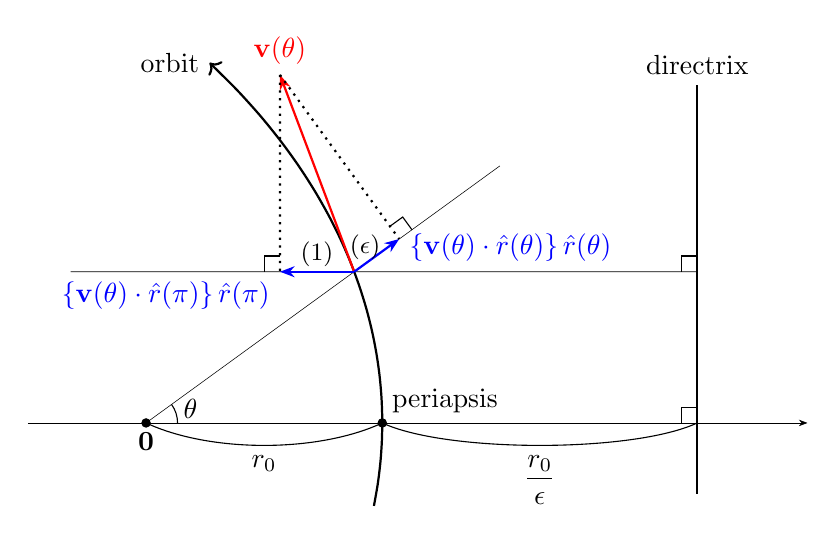
\begin{tikzpicture}[scale=3]
  \def \rightanglesymsize {0.1}

  \def \gm {0.5}  % gravatity coefficeient
  \def \e {0.75}  % eccentricity
  \def \rz {1}   % distance at periapsis
  
  \def \vz {sqrt((1 + \e) * \gm / \rz)}  % speed at periapsis
  \def \l {(1 + \e) * \rz}  % Semi latus rectum

  % Origin 
  \coordinate (O) at (0, 0);
  \filldraw[black] (O) circle (0.5pt) node[anchor=north] {$\vcz$};

  % Periapsis line
  \draw[very thin,vechead] (-0.5, 0) -- ({1.2 * (1 + 1/\e) * \rz}, 0) coordinate (G);

  % Periapsis
  \filldraw[black] (\rz, 0) circle (0.5pt) node[anchor=south west] {periapsis};
  \draw[thin] (0, 0) to [out=335,in=205,distance=0.3cm] 
    node[anchor=midway,below] {$r_0$} (\rz, 0);

  % Orbit
  \draw[thick,->] plot [variable=\t,domain=-20:80,smooth,samples=20] 
    ({\l / (1 + \e * cos(\t)) * cos(\t)}, {\l / (1 + \e * cos(\t)) * sin(\t)}) node[anchor=east] {orbit};

  \foreach \phi in {pi/5} {
      % Planet position
      \coordinate (p) at ({\l / (1 + \e * cos(\phi r)) * cos(\phi r)}, {\l / (1 + \e * cos(\phi r)) * sin(\phi r)});

      % Directrix line
      \draw[thick] ({(1 + 1/\e) * \rz}, -0.3) -- ({(1 + 1/\e) * \rz}, 0) coordinate (I) -- ({(1 + 1/\e) * \rz}, 1.43) coordinate (H) node[anchor=south] {directrix};
      \draw[thin] (\rz, 0) .. controls +(335:0.3) and +(205:0.3) ..
        node[anchor=midway,below] {$\displaystyle\frac{r_0}{\epsilon}$} ({(1 + 1 / \e) * \rz}, 0);
    
      % Radial line
      \draw[very thin] (0, 0) -- ($1.7*(p)$) coordinate (C);

      % Horizontal line through planet
      \draw[very thin] ($(p)+(-1.2,0)$) coordinate (F) -- ({(1 + 1/\e) * \rz}, {\l / (1 + \e * cos(\phi r)) * sin(\phi r)}) coordinate (J);
      
      % Velocity vector
      \coordinate (v) at ({(\gm / (\rz * \vz) * (-sin(\phi r))) }, {(\gm / (\rz * \vz) * (\e + cos(\phi r))) });
      \draw[red,thick,vechead] (p) -- ++(v) node[anchor=south,xshift=0,yshift=0] {$\vc{v}(\theta)$};
    
      % Radial component
      \def \radialcomponent {((\gm / (\rz * \vz) * (-sin(\phi r))) * cos(\phi r) + (\gm / (\rz * \vz) * (\e + cos(\phi r))) * sin(\phi r))}
      % \draw[thin] (p) to [out=335,in=245,distance=0.5mm] node[anchor=midway,right,xshift=-6,yshift=-6] {$(\epsilon)$} 
        % ++({\radialcomponent * cos(\phi r)}, {\radialcomponent * sin(\phi r)});
      \draw[blue,thick,vechead] (p) -- node[black,anchor=midway,left,xshift=5,yshift=3] {$\text{\small ($\epsilon$)}$} ++({\radialcomponent * cos(\phi r)}, {\radialcomponent * sin(\phi r)}) 
        node[anchor=west,yshift=-3] {$\{\vc{v}(\theta) \cdot \hat{r}(\theta)\}\,\hat{r}(\theta)$};
    
      % Horizontal component
      \def \horizontalcomponent {((\gm / (\rz * \vz) * (sin(\phi r)))}
      % \draw[thin] (p) to [out=205,in=335,distance=0.1cm] node[anchor=midway,below,yshift=2] {$(1)$} ++({-\horizontalcomponent}, 0);
      \draw[blue,thick,vechead] (p) -- node[black,anchor=midway,above,yshift=-2] {$\text{\small ($1$)}$} ++({-\horizontalcomponent}, 0) node[anchor=north east] {$\{\vc{v}(\theta) \cdot \hat{r}(\pi)\}\,\hat{r}(\pi)$};
    
      % Two perpendicular dotted lines
      \draw[thick,dotted] ($(p)+(v)$) coordinate (A) -- ($(p)+({\radialcomponent * cos(\phi r)}, {\radialcomponent * sin(\phi r) })$) coordinate (B);
      \draw[thick,dotted] ($(p)+(v)$) coordinate (D) -- ($(p)+({-\horizontalcomponent}, 0)$) coordinate (E);
      
      \draw pic [draw,angle radius=2mm] {right angle = A--B--C};
      \draw pic [draw,angle radius=2mm] {right angle = D--E--F};
      \draw pic [draw, angle radius=2mm] {right angle = H--I--O};
      \draw pic [draw, angle radius=2mm] {right angle = H--J--p};

      \draw pic [draw,angle radius=4mm] {angle = G--O--C};
      \draw (O) node[anchor=south west,xshift=10,yshift=-2] {$\theta$};
  }
\end{tikzpicture}

\caption{Kepler's first law: The proof is completely encoded in the fact that the ratio
$\displaystyle\frac{\vc{v}(\theta)\cdot\hat{r}(\theta)}{\vc{v}(\theta)\cdot\hat{r}(\pi)}=\epsilon$
is independent of $\theta$.}

\end{center}
\end{figure}

\newcommand{\Hodograph}[2]{
  \begin{tikzpicture}[scale=2.8]
    \def \gm {0.5} % gravitational constant factor
    \def \e {#1}   % eccentricity
    \def \rz {1}   % distance at periapsis
    
    \def \vz {sqrt((1 + \e) * \gm / \rz)} % speed at periapsis
    \def \tz {#2 * 0.2} % 표시 각도 스케일
    
    % 좌표축
    \draw[vechead] (-0.7, 0) -- (0.7, 0);
    \draw[vechead] (0, -0.2) node[anchor=north] {$(\epsilon=#1)$} -- (0, 1.2) coordinate (A);
    
    % Hodograph 곡선
    \draw[blue,very thick] plot [variable=\t,domain=-#2:#2,smooth,samples=20] 
    ({(\gm / (\rz * \vz) * (-sin(\t)))}, {(\gm / (\rz * \vz) * (\e + cos(\t)))});
    
    % 여러 속도 벡터
    \foreach \i [evaluate=\i as \phi using #2*\i] in {-1,-0.8,...,1} {
        \draw[thin,vechead] (0, 0) -- ({(\gm / (\rz * \vz) * (-sin(\phi)))}, {(\gm / (\rz * \vz) * (\e + cos(\phi)))});
    }
    
    % 중심 점 표시
    \filldraw[black] (0, {\gm / (\rz * \vz) * \e}) coordinate (C) circle (0.3pt) 
        node[anchor=west] {$\frac{GM}{r_0 v_0}(0,\epsilon)$};
    
    % 각도 표시
    \draw[blue] (0, {\gm / (\rz * \vz) * \e}) -- ++($1.2 * \gm / (\rz * \vz)*({-sin(\tz)}, {cos(\tz)})$) coordinate (B);
    \draw[red,thick,vechead] (0, 0) -- ({(\gm / (\rz * \vz) * (-sin(\tz)))}, {(\gm / (\rz * \vz) * (\e + cos(\tz)))}) node[anchor=east] {$\vc{v}(\theta)$};
    
    \draw pic [red,draw,angle radius=3mm] {angle = A--C--B};
    \draw (C) node[red,anchor=south east,xshift=2,yshift=6] {$\theta$};
    
    % 벡터 라벨
    \draw[thick,blue] (0, {\gm / (\rz * \vz) * \e}) to [out=335,in=25,distance=0.5mm] node[anchor=midway,right] {$(\epsilon)$} (0, 0);
    \draw[thick,blue] (0, {\gm / (\rz * \vz) * \e}) to [out=25,in=335,distance=0.7mm] node[anchor=midway,right] {$(1)$} (0, {\gm / (\rz * \vz) * (\e + 1)});
  \end{tikzpicture}
}

\begin{figure}[h!]
    \centering
    \Hodograph{0.75}{180}
    \Hodograph{1}{180}
    \Hodograph{1.5}{180} % 초과값은 acos(-1/\e) 등으로 조정 가능
    \caption{Hodographs for the cases $\epsilon=0.75$, $\epsilon=1$, and $\epsilon=1.5$.}
\end{figure}

\newpage

\section{Figures in `Uniqueness of non-Euclidean Mass Center System and Generalized Pappus' Centroid Theorems in Three Geometries' (arXiv:2412.03080)}

\begin{figure}[h!]
    \begin{center}
        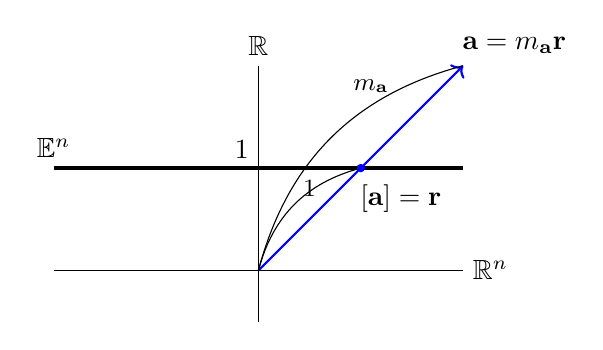
\begin{tikzpicture}[scale=1.3]
          % draw axes
          \draw (0, -0.5) -- (0, 2) node[anchor=south]{$\mathbb{R}$};
          \draw (-2,0) -- (2,0) node[anchor=west]{$\mathbb{R}^n$};
        
          \draw (0,1) node[anchor=south east]{$1$};
        
          % plot
          \draw[very thick] (-2,1) node[anchor=south]{$\mathbb{E}^n$}  -- (2,1);
          \draw[blue, thick, ->] (0,0) -- (2,2);
        
          \draw (0,0) to [bend left=30] (1,1);
          \draw (0.5,0.8) node {\small $1$};
        
          \draw (0,0) to [bend left=30] (2,2);
          \draw (1.1,1.8) node {\small $m_{\vc a}$};
        
          \filldraw[blue] (1,1) circle (1pt);
          \draw (2.5, 2.2) node {$\vc a = m_{\vc a}\vc r$};
          \draw (0.9,0.7) node[anchor=west] {$[\vc a] = \vc r$};
        \end{tikzpicture}
        
        \caption{Euclidean Space $\mathbb{E}^n$ lying on the ambient space $\mathbb{R}^{n+1}$, a material point $[\vc a]$ with mass $m_{\vc a}$, and the corresponding material vector $\vc a$. The concepts of material point, mass, and material vector will be introduced in the following section. }\label{efig1}
    \end{center}
\end{figure}

\begin{figure}[h!]
    \begin{center}
        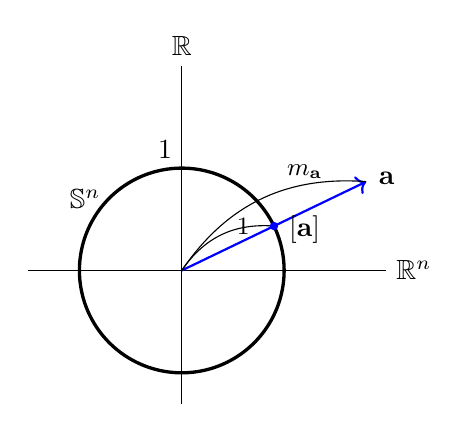
\begin{tikzpicture}[scale=1.3]
          % draw axes
          \draw (0, -1.3) -- (0, 2) node[anchor=south]{$\mathbb{R}$};
          \draw (-1.5,0) -- (2,0) node[anchor=west]{$\mathbb{R}^n$};
        
          \draw (0,1) node[anchor=south east]{$1$};
        
          % plot
          \draw[very thick, domain=0:360, smooth, variable=\t, samples=100] 
            plot ({cos(\t)}, {sin(\t)});
        
          \draw (-0.7, 0.7) node[anchor=east]{$\mathbb{S}^n$};
        
          \draw[blue, thick, ->, trig format=rad] (0,0) -- ({2*cos(pi/7)}, {2*sin(pi/7)});
        
          \draw (0,0) to [bend left=30] ({cos(deg(pi/7))}, {sin(deg(pi/7))});
          \draw (0.6,{sin(deg(pi/7))}) node {\small $1$};
        
          \draw (0,0) to [bend left=30] ({2*cos(deg(pi/7))}, {2*sin(deg(pi/7))});
          \draw (1.2,{2*sin(deg(pi/7))+0.1}) node {\small $m_{\vc a}$};
        
          \filldraw[blue] ({cos(deg(pi/7))}, {sin(deg(pi/7))}) circle (1pt);
          \draw (2, 0.9) node { $\vc a$};
          \draw (1.2, 0.4) node { $[\vc a]$};
        \end{tikzpicture}
        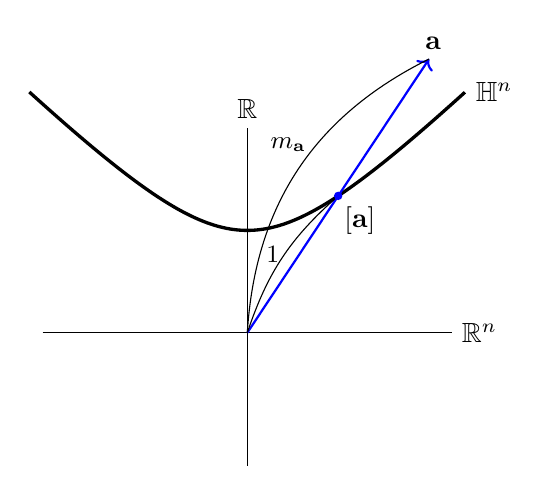
\begin{tikzpicture}[scale=1.3]
          % draw axes
          \draw (0, -1.3) -- (0, 2) node[anchor=south]{$\mathbb{R}$};
          \draw (-2,0) -- (2,0) node[anchor=west]{$\mathbb{R}^n$};
        
          \draw[very thick, domain=-1.5:1.5, smooth, variable=\t, samples=100] 
            plot ({sinh(\t)}, {cosh(\t)}) node[anchor=west]{$\mathbb{H}^n$};
          % \draw[domain=-1.5:2, smooth, variable=\x] plot ({\x}, {\x});
          % \draw[domain=-2:1.5, smooth, variable=\x] plot ({\x}, {-\x});
        
          \draw[blue, thick, ->, trig format=rad] (0,0) -- ({2*sinh(0.8)}, {2*cosh(0.8)});
        
          \draw (0,0) to [bend left=15] ({sinh(0.8)}, {cosh(0.8)});
          \draw (0.25,{0.5*cosh(0.8)+0.1}) node {\small $1$};
        
          \draw (0,0) to [bend left=30] ({2*sinh(0.8)}, {2*cosh(0.8)});
          \draw (0.4,{cosh(0.8)+0.5}) node {\small $m_{\vc a}$};
        
          \draw ({2*sinh(0.75)}, {2*cosh(0.8)}) node[anchor=south west] { $\vc a$};
          \filldraw[blue] ({sinh(0.8)}, {cosh(0.8)}) circle (1pt);
          \draw (1.1, 1.1) node { $[\vc a]$};
        \end{tikzpicture}

        \caption{Spherical Space $\mathbb{S}^n$ and hyperbolic space $\mathbb{H}^n$ lying on the ambient space $\mathbb{R}^{n+1}$, material points $[\vc a]$ with mass $m_{\vc a}$, and the corresponding material vectors $\vc a$}\label{efig2}
    \end{center}
\end{figure}

\begin{figure}[h!]
    \vspace{1cm}
		\begin{center}
			%\includegraphics[width=5cm]{cone3.jpg}
            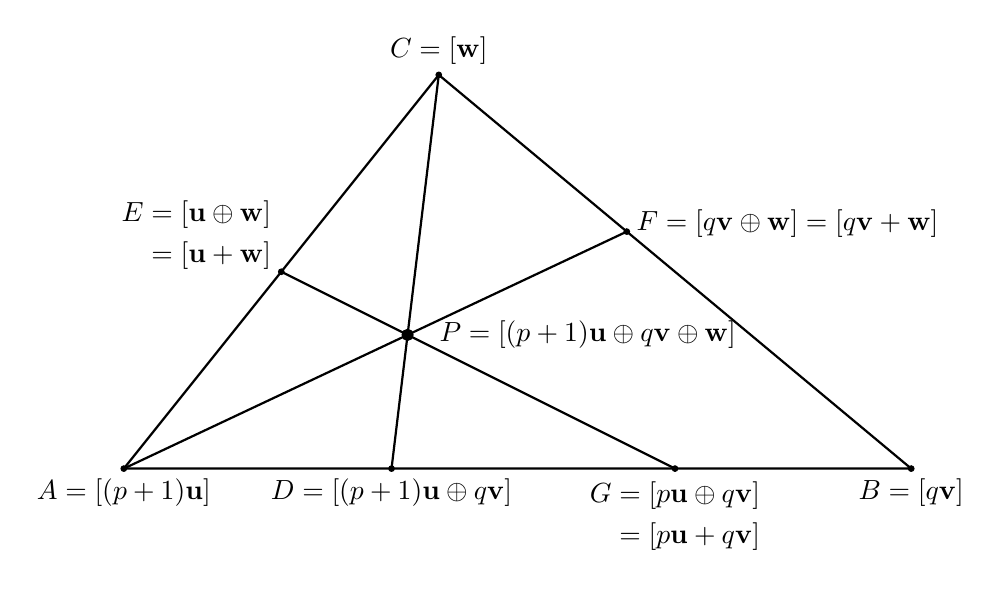
\begin{tikzpicture}
              \coordinate (A) at (0, 0);
              \coordinate (B) at (10, 0);
              \coordinate (C) at (4, 5);
              \coordinate (D) at (3.4, 0);
              \coordinate (E) at (2, {1.25*2});
              \coordinate (G) at (7, 0);
            
              \draw[thick] (A) node[anchor=north] {$A = [(p + 1) \vc{u}]$}
                -- (B) node[anchor=north] {$B = [q \vc{v}]$}
                -- (C) node[anchor=south] {$C = [\vc{w}]$} 
                -- cycle;
            
              \draw[thick, name path=C--D] (C) 
                -- (D) node[anchor=north] {$D = [(p + 1) \vc{u} \oplus q \vc{v}]$};
            
              \draw[thick, name path=E--G] (E) node[anchor=south east, yshift=-4] 
                {$\begin{aligned}
                    E = [\vc {u} \oplus \vc {w}]\\ = [\vc {u} + \vc {w}]
                \end{aligned}$}
                -- (G) node[anchor=north] {$\begin{aligned}
                  G = [p \vc{u} \oplus q \vc{v}]\\ = [p \vc{u} + q \vc{v}]
                \end{aligned}$};
            
              \filldraw[black] (A) circle (1pt)
                (B) circle (1pt)
                (C) circle (1pt)
                (D) circle (1pt)
                (E) circle (1pt)
                (G) circle (1pt);
            
              \coordinate (P) at (intersection of C--D and E--G);
              \filldraw[black] (P) circle (2pt)
                node[anchor=west, xshift=8] {$P = [(p + 1) \vc{u} \oplus q \vc{v} \oplus \vc{w}]$};
            
              \path[name path=A--P] (A) -- (P);
              \path[name path=B--C] (B) -- (C);
              \coordinate (F) at (intersection of A--P and B--C);
            
              \filldraw[black] (F) circle (1pt) 
                node[anchor=west, yshift=3] {$F = [q \vc{v} \oplus \vc{w}] 
                  = [q \vc{v} + \vc{w}]$};
              \draw[thick] (A) -- (F);
            \end{tikzpicture}
           \caption{concurrent segments $\overline{AF}$, $\overline{CD}$, $\overline{EG}$ and the induction hypothesis applied on the points $E$, $F$, $G$  }\label{fig:triangleabc}
		\end{center}
\end{figure}

\begin{figure}[h!]
    \begin{center}
        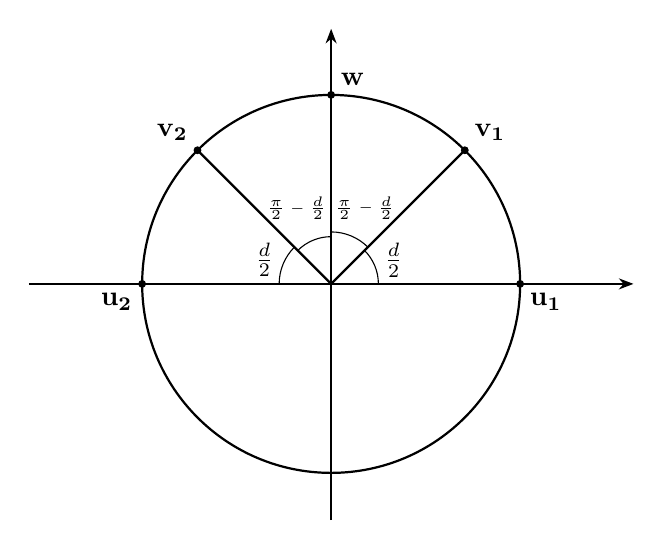
\begin{tikzpicture}[scale=1.2]
          \def \r {2} % radius
        
          \coordinate (u1) at (\r, 0);
          \coordinate (u2) at (-\r, 0);
          \coordinate (v1) at ({\r * cos(45)}, {\r * sin(45)});
          \coordinate (v2) at ({\r * cos(135)}, {\r * sin(135)});
          \coordinate (w) at (0, \r);
        
          \draw[vechead, thick] (-3.2, 0) -- (3.2, 0);
          \draw[vechead, thick] (0, -2.5) -- (0, 2.7);
          \draw[thick] circle (\r);
        
          \filldraw[black] (u1) circle (1pt)
            node[anchor=north west] {$\vc{u_1}$};
          \filldraw[black] (u2) circle (1pt)
            node[anchor=north east] {$\vc{u_2}$};
          \filldraw[black] (v1) circle (1pt)
            node[anchor=south west] {$\vc{v_1}$};
          \filldraw[black] (v2) circle (1pt)
            node[anchor=south east] {$\vc{v_2}$};
          \filldraw[black] (w) circle (1pt)
            node[anchor=south west] {$\vc{w}$};
        
          \draw[thick] (0, 0) -- (v1);
          \draw[thick] (0, 0) -- (v2);
        
          \draw (0.5, 0) arc (0:45:0.5) node[midway, anchor=west, yshift=2] {$\frac{d}{2}$};
          \draw ({0.55 * cos(45)}, {0.55 * sin(45)}) arc (45:90:0.55) node[midway, anchor=south, xshift=5, yshift=2.5] 
              {\tiny{$\frac{\pi}{2} - \frac{d}{2}$}};
          \draw (0, 0.5) arc (90:135:0.5) node[midway, anchor=south, xshift=-6, yshift=4]
              {\tiny{$\frac{\pi}{2} - \frac{d}{2}$}};
          \draw (-0.55, 0) arc (180:135:0.55) node[midway, anchor=east, yshift=1.5] {$\frac{d}{2}$};
        \end{tikzpicture}
        \caption{five material points on $\mathbb{S}^1$}\label{fig:circle77}
    \end{center}
\end{figure}

\begin{figure}[h!]
    \begin{center}\label{fig:2277}
        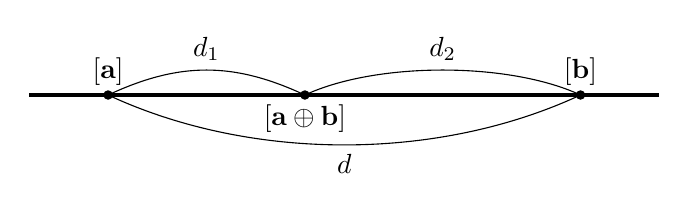
\begin{tikzpicture}
          \coordinate (A) at (1, 0);
          \coordinate (B) at (7, 0);
          \coordinate (P) at (3.5, 0);
          
          \draw[very thick] (0, 0) -- (8, 0);
          \filldraw[black] (A) circle (1.5pt) node[anchor=south] {$[\vc {a}]$};
          \filldraw[black] (B) circle (1.5pt) node[anchor=south] {$[\vc {b}]$};
          \filldraw[black] (P) circle (1.5pt) node[anchor=north] {$[\vc {a} \oplus \vc {b}]$};
          
          \draw (A) to [out=25, in=155, distance=1cm] node[midway, above] {$d_1$} (P);
          \draw (P) to [out=25, in=155, distance=1cm] node[midway, above] {$d_2$} (B);
          \draw (A) to [out=155, in=25, distance=-2cm] node[midway, below] {$d$} (B);
        \end{tikzpicture}
        \caption{two material points and their mass center}
    \end{center}
\end{figure}

\begin{figure}[h!]
    \centering
    \begin{subfigure}[b]{0.45\linewidth}
        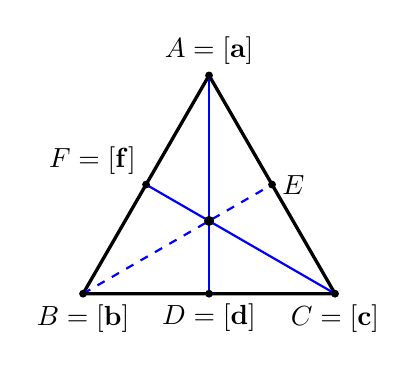
\begin{tikzpicture}[scale=0.8]
          \coordinate (A) at (0, {2*sqrt(3)});
          \coordinate (B) at (-2, 0);
          \coordinate (C) at (2, 0);
          \coordinate (D) at (0, 0);
          \coordinate (E) at (1, {sqrt(3)});
          \coordinate (F) at (-1, {sqrt(3)});
          \coordinate (P) at (0, {2*sqrt(3)/3});
          \draw[very thick]
               (A) node[anchor=south]{$A = [\vc{a}]$}
            -- (B) node[anchor=north]{$B = [\vc{b}]$}
            -- (C) node[anchor=north]{$C = [\vc{c}]$}
            -- cycle;
          \draw[thick, blue]
              (A) -- (D) node[anchor=north, black]{$D = [\vc{d}]$};
          \draw[thick, dashed, blue]
              (B) -- (E) node[anchor=west, black]{$E$};
          \draw[thick, blue]
              (C) -- (F) node[anchor=south east, black]{$F = [\vc{f}]$};
          \filldraw[black] (P) circle (2pt);
        
          \filldraw[black] (A) circle (1.5pt)
            (B) circle (1.5pt) 
            (C) circle (1.5pt)
            (D) circle (1.5pt)
            (E) circle (1.5pt)
            (F) circle (1.5pt);
        \end{tikzpicture}
        \caption{CASE 1}
    \end{subfigure}
    \begin{subfigure}[b]{0.45\linewidth}
        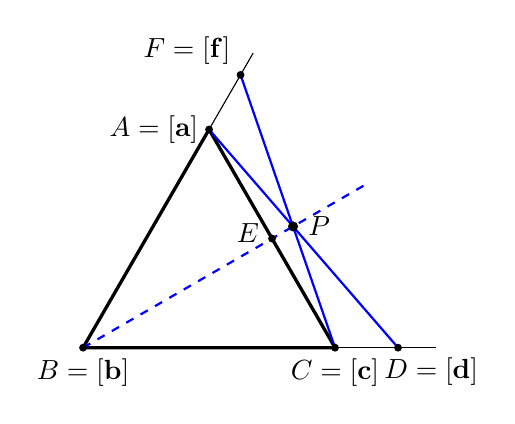
\begin{tikzpicture}[scale=0.8]
          \coordinate (A) at (0, {2*sqrt(3)});
          \coordinate (B) at (-2, 0);
          \coordinate (C) at (2, 0);
          \coordinate (D) at (3, 0);
          \coordinate (D') at (3.6, 0);
          \coordinate (E) at (1, {sqrt(3)});
          \coordinate (E') at (3-0.5, {(5-0.5)*sqrt(3)/3});
          \coordinate (F) at (0.5, {2.5*sqrt(3)});
          \coordinate (F') at (1-0.3, {(3-0.3)*sqrt(3)});
          \draw[very thick]
               (A) node[anchor=east]{$A = [\vc{a}]$}
            -- (B) node[anchor=north]{$B = [\vc{b}]$}
            -- (C) node[anchor=north]{$C = [\vc{c}]$}
            -- cycle;
          \draw[thick, name path=AD, blue]
               (A) -- (D) node[anchor=north, xshift=12, black]{$D = [\vc{d}]$};
          \draw[thick, dashed, blue]
               (B) -- (E) node[anchor=east, xshift=-1, yshift=2, black]{$E$} -- (E');
          \draw[thin](A) -- (F');
          \draw[thin](C) -- (D');
          \draw[thick, name path=CF, blue]
              (C) -- (F) node[anchor=south east, black]{$F = [\vc{f}]$};
          \filldraw[black, name intersections={of=AD and CF}] 
            (intersection-1) circle (2pt) node[anchor=west, xshift=2] {$P$};
        
          \filldraw[black] (A) circle (1.5pt)
            (B) circle (1.5pt) 
            (C) circle (1.5pt)
            (D) circle (1.5pt)
            (E) circle (1.5pt)
            (F) circle (1.5pt);
        \end{tikzpicture}
        \caption{CASE 2}
    \end{subfigure}
    \caption{[Ceva's theorem] Masses are placed on $A=[\vc{a}]$, $B=[\vc{b}]$, $C=[\vc{c}]$ so that $\vc{f}=\vc{a}\oplus\vc{b}$, $\vc{d}=\vc{b}\oplus\vc{c}$ (CASE 1)   or $\vc{a}=\vc{b}\oplus\vc{f}$, $\vc{c}=\vc{b}\oplus\vc{d}$ (CASE 2).}
    \label{figceva}
\end{figure}

\begin{figure}[h!]
    \centering
    \begin{subfigure}[b]{0.4\linewidth}
        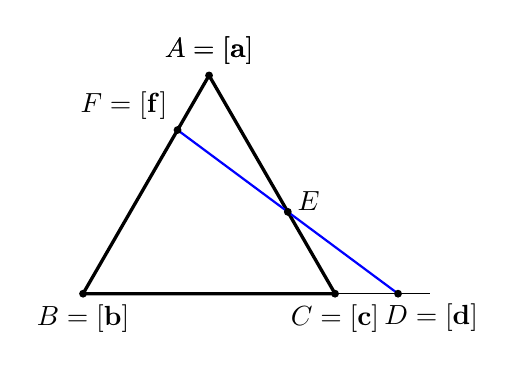
\begin{tikzpicture}[scale=0.8]
          \coordinate (A) at (0, {2*sqrt(3)});
          \coordinate (B) at (-2, 0);
          \coordinate (C) at (2, 0);
          \coordinate (D) at (3, 0);
          \coordinate (D') at (3.5, 0);
          \coordinate (E) at (1, {sqrt(3)});
          \coordinate (F) at (-0.5, {1.5*sqrt(3)});
        
          \draw[very thick]
                 (A) node[anchor=south]{$A = [\vc{a}]$}
              -- (B) node[anchor=north]{$B = [\vc{b}]$}
              -- (C);
          \draw[thin] (C) -- (D);
        
          \draw[very thick, name path=AC]
               (C) node[anchor=north]{$C = [\vc{c}]$}
            -- (A) node[anchor=south]{$A = [\vc{a}]$};
          \draw[thick, blue, name path=DF]
               (F) node[anchor=south east, black]{$F = [\vc{f}]$}
            -- (D) node[anchor=north, black, xshift=12]{$D = [\vc{d}]$};
          \draw[thin] (D) -- (D');
          \filldraw[black, name intersections={of=AC and DF}]
            (intersection-1) circle (1.5pt) node[anchor=west, yshift=4]{$E$};
        
          \filldraw[black] (A) circle (1.5pt)
            (B) circle (1.5pt) 
            (C) circle (1.5pt)
            (D) circle (1.5pt)
            (F) circle (1.5pt);
        \end{tikzpicture}
        \caption{CASE 3}
    \end{subfigure}
    \hspace{2em}
    \begin{subfigure}[b]{0.4\linewidth}
        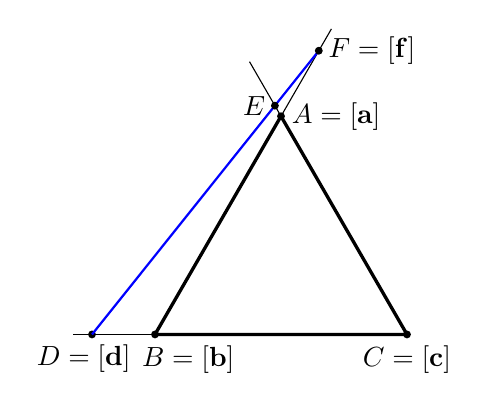
\begin{tikzpicture}[scale=0.8]
          \coordinate (A) at (0, {2*sqrt(3)});
          \coordinate (B) at (-2, 0);
          \coordinate (C) at (2, 0);
          \coordinate (D) at (-3, 0);
          \coordinate (D') at (-3.3, 0);
          %\coordinate (E) at (1, {sqrt(3)});
          \coordinate (E') at (-0.5,{(2+0.5)*sqrt(3)});
          \coordinate (F) at (0.6, {(2+0.6)*sqrt(3)});
          \coordinate (F') at (0.8, {(2+0.8)*sqrt(3)});
          \draw[very thick]
              (A) node[anchor=west]{$A = [\vc{a}]$}
              -- (B) node[anchor=north, xshift=12]{$B = [\vc{b}]$}
              -- (C) node[anchor=north]{$C = [\vc{c}]$} 
              -- cycle;
          \filldraw[black] (A) circle (1.5pt)
            (B) circle (1.5pt) 
            (C) circle (1.5pt)
            (D) circle (1.5pt);
          
          \draw[thin, name path=F'A] (F') -- (A);
          \draw[thin] (D') -- (B);
          \draw[thin, name path=E'A] (E') -- (A);
          \draw[thick, name path=DF, blue]
               (F) -- (D) node[anchor=north, xshift=-3, black]{$D = [\vc{d}]$};
          \filldraw[black, name intersections={of=E'A and DF}]
            (intersection-1) circle (1.5pt) node[anchor=east]{$E$};
          \filldraw[black, name intersections={of=F'A and DF}] 
            (intersection-1) circle (1.5pt) node[anchor=west]{$F = [\vc{f}]$};
        \end{tikzpicture}
        \caption{CASE 4}
    \end{subfigure}
    \caption{[Menelaus' theorem] Masses are placed on $A=[\vc{a}]$, $B=[\vc{b}]$, $C=[\vc{c}]$ so that $\vc{f}=\vc{a}\oplus\vc{b}$, $\vc{c}=\vc{b}\oplus\vc{d}$ (CASE 3)   or $\vc{a}=\vc{b}\oplus\vc{f}$, $\vc{b}=\vc{c}\oplus\vc{d}$ (CASE 4).}
    \label{figmenelaus} 
\end{figure}

\begin{figure}[h!]
    \begin{center}
        \begin{subfigure}[c]{0.45\textwidth}
            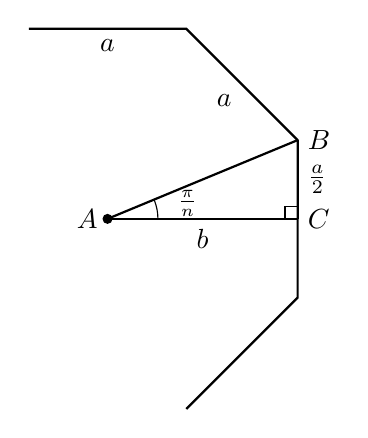
\begin{tikzpicture}[scale=0.8]
              \def \a {2.5}
              \def \b {(\a/2 + \a/sqrt(2))}
            
              \coordinate (A) at (0, 0);
              \coordinate (B) at ({\b}, {\a/2});
              \coordinate (C) at ({\b}, 0);
            
              \draw[thick] ({\b - \a * cos(45) - \a}, {\a/2 + \a * sin(45)}) 
                -- ({\b - \a * cos(45)}, {\a/2 + \a * sin(45)}) node[midway, anchor=north] {$a$}
                -- (B) node[midway, anchor=north east] {$a$}
                -- ({\b}, -{\a/2})
                -- ({\b - \a * cos(45)}, {-\a/2 - \a * sin(45)});
            
              \draw[thick] (A) -- (B) node[anchor=west] {$B$};
              \draw[thick] (A) -- (C) node[midway, anchor=north] {$b$} 
                                      node[anchor=west] {$C$};
              \draw[thick] (B) -- (C) node[midway, anchor=west] {$\frac{a}{2}$};
             
              \draw ({\b - 0.2}, 0) -- ({\b - 0.2}, 0.2) -- ({\b}, 0.2); % right angle sign
              \draw (0.8, 0) arc (0:{atan((\a/2)/\b)}:0.8) 
                node[midway, anchor=west, xshift=4, yshift=2] {\small$\frac{\pi}{n}$};
              
              \filldraw[black] (A) circle (2pt)
                node[anchor=east] {$A$};
            \end{tikzpicture}
        \end{subfigure}
        \hspace{-30pt}
        \begin{subfigure}[c]{0.45\textwidth}
            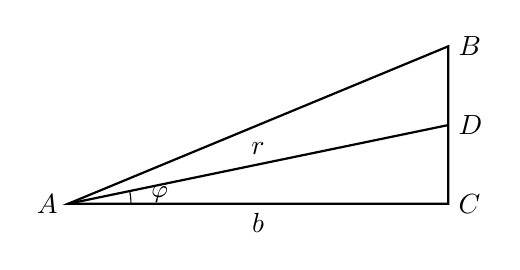
\begin{tikzpicture}
              \def \a {4}
              \def \b {(\a/2 + \a/sqrt(2))}
            
              \coordinate (A) at (0, 0);
              \coordinate (B) at ({\b}, {\a/2});
              \coordinate (C) at ({\b}, 0);
              \coordinate (D) at ({\b}, {\a/4});
            
              \draw[thick] (A) node[anchor=east] {$A$}
                -- (B) node[anchor=west] {$B$} 
                -- (C) node[anchor=west] {$C$} 
                -- cycle;
            
              \draw (A) -- (C) node[midway, anchor=north] {$b$};
              \draw[thick] (A) -- (D) node[midway, anchor=south] {$r$}
                                      node[anchor=west] {$D$};
            
              \draw (0.8, 0) arc (0:{atan((\a/2/2)/\b)}:0.8) node[midway, anchor=west, xshift=4, yshift=1] {\small{$\varphi$}};
            \end{tikzpicture}
        \end{subfigure}
        \caption{a spherical or hyperbolic regular $n$-gon}\label{regu2277}
    \end{center}
\end{figure}

\begin{figure}[h!]
    \begin{center}\label{fig:2266}
        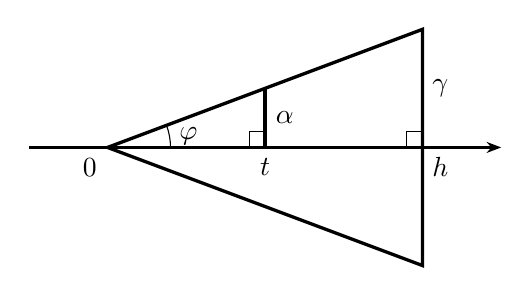
\begin{tikzpicture}
          \coordinate (A) at (0, 0);
          \coordinate (B) at (4, 1.5);
          \coordinate (C) at (4, -1.5);
          \coordinate (D) at (2, {2 * 1.5/4});
        
          \draw[vechead, thick] (-1, 0) -- (5, 0);
        
          \draw[very thick] (A) node[anchor=north east] {$0$}
            -- (B)
            -- (C) 
            -- cycle;
          \draw[very thick] (D) -- (2, 0) node[midway, anchor=west] {$\alpha$}
                                          node[anchor=north] {$t$};
        
          \draw (B) -- (4, 0) node[midway, anchor=west] {$\gamma$} 
                              node[anchor=north west] {$h$};
        
          \draw (0.8, 0) arc (0:20.5:0.8) node[midway, anchor=west] {$\varphi$};
          \draw ({2 - 0.2}, 0) -- ({2 - 0.2}, 0.2) -- (2, 0.2);
          \draw ({4 - 0.2}, 0) -- ({4 - 0.2}, 0.2) -- (4, 0.2);
        \end{tikzpicture}
        \caption{the triangular cross-section passing through the apex of a right circular cone}
    \end{center}
\end{figure}

\begin{figure}[h!]
    \begin{center}\label{fig:10}
        \tdplotsetmaincoords{65}{40}
          \begin{tikzpicture}[scale=1.5, tdplot_main_coords]
            \def \a {3}
            \def \b {(\a/2 + \a/sqrt(2))}
            \def \h {\a}
        
            \coordinate (A) at (0, 0, 0);
            \coordinate (B) at ({\b}, {\a/2}, 0);
            \coordinate (C) at ({\b}, 0, 0);
            \coordinate (O) at (0, 0, {\h});
        
            \coordinate (A') at (0, 0, {\h/2});
            \coordinate (B') at ({\b/2}, {\a/4}, {\h/2});
            \coordinate (C') at ({\b/2}, 0, {\h/2});
        
            % dots and signs
            % right angle signs have a width and height of w
            \def \w {0.2}
            
            % Exception: right angle signs of OCB and OC'B' 
            % have a height of wh
            \def \wh {(0.2 * sin(atan(\a/\b)) - 0.03)}
        
            \draw (O) to [bend right=40] node[midway, fill=white] {$t$} (A');
            \draw (O) to [bend right=40] node[midway, fill=white] {$h$} (A);
        
            \filldraw[blue] (A) circle (1.2pt);
        
            % BCA, B'C'A'
            \draw[blue] ({\b - \w}, 0) -- ({\b - \w}, \w) -- ({\b}, \w);
            \draw[blue] ({\b/2 - \w}, 0, {\h/2}) 
             -- ({\b/2 - \w}, \w, {\h/2}) 
             -- ({\b/2}, \w, {\h/2});
        
            % OCB, OC'B'
            \draw[blue] ({\b}, \w) 
              -- ({\b - \wh}, \w, {\h/\b * \wh})
              -- ({\b - \wh}, 0, {\h/\b * \wh});
            \draw[blue] ({\b/2}, \w, {\h/2}) 
              -- ({\b/2 - \wh}, \w, {\h/2 + \h/\b * \wh})
              -- ({\b/2 - \wh}, 0, {\h/2 + \h/\b * \wh});
        
            % OAC, OA'C'
            \draw[blue] (\w, 0, 0) -- (\w, 0, \w) -- (0, 0, \w);
            \draw[blue] (\w, 0, {\h/2}) -- (\w, 0, {\h/2 + \w}) -- (0, 0, {\h/2 + \w});
         
            % pyramid
            \draw[blue, thick, dashed] (A) node[black, anchor=east, xshift=-2] {$A$}
              -- (B) node[black, anchor=west] {$B$};
            \draw[blue, thick] (B) -- (C) node[black, midway, anchor=west, yshift=-5] {$\frac{a}{2}$}
                                          node[black, anchor=west, yshift=-4] {$C$};
            \draw[blue, thick] (C) -- (A) node[black, midway, anchor=north] {$b$};
        
            \draw[blue, thick] (A) -- (O) node[black,, anchor=south] {$O$};
            \draw[blue, thick] (B) -- (O);
            \draw[blue, thick] (C) -- (O);
        
            % using cycle makes the points of the triangle stick out of the pyramid.
            \draw[blue, thick, dashed] (A') -- (B') node[black, anchor=south, xshift=6, yshift=-2] {$B'$};
            \draw[blue, thick] (B') -- (C') node[black, midway, anchor=west, xshift=-2, yshift=-6] 
                                              {$\frac{\gamma}{2}$} 
                                            node[black, anchor=north, xshift=-5, yshift=2] {$C'$};
            \draw[blue, thick] (C') -- (A') node[black, midway, anchor=north] {$\alpha$}
                                            node[black, anchor=east] {$A'$}; 
        
            % polygon
            \draw[thick] ({\b - \a * cos(45)}, {\a/2 + \a * sin(45)})
            -- (B)
            -- ({\b}, -{\a/2})
            -- ({\b - \a * cos(45)}, {-\a/2 - \a * sin(45)});
          \end{tikzpicture}
        \caption{a spherical or hyperbolic right cone with a regular $n$-gonal base}
    \end{center}
\end{figure}

\end{document}
